% 三角形中位线定理 + 倍长中位线证明构造
% △ABC, D,E 为 AB,AC 中点；延长 DE 到 F 使 EF=DE；连接 CF
\documentclass[tikz,border=4pt]{standalone}
\usepackage{ctex}
\usepackage{amsmath}
\usetikzlibrary{calc, decorations.markings}
\begin{document}
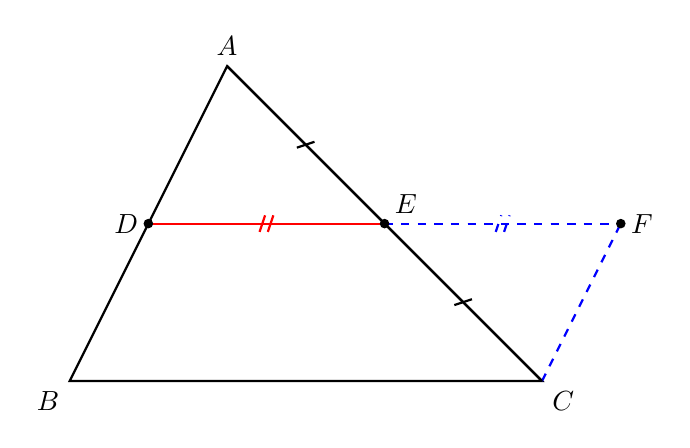
\begin{tikzpicture}[
  scale=1.0, thick,
  tickone/.style={postaction={decorate, decoration={markings,
    mark=at position 0.5 with {\draw (-1.5pt,-3pt) -- (1.5pt,3pt);}}}},
  ticktwo/.style={postaction={decorate, decoration={markings,
    mark=at position 0.5 with {\draw (-2.5pt,-3pt) -- (-0.5pt,3pt);
                               \draw (0.5pt,-3pt)  -- (2.5pt,3pt);}}}},
]
  \coordinate (A) at (2,4);
  \coordinate (B) at (0,0);
  \coordinate (C) at (6,0);
  \coordinate (D) at ($(A)!0.5!(B)$);
  \coordinate (E) at ($(A)!0.5!(C)$);
  % F 在 DE 延长线上，EF=DE
  \coordinate (F) at ($(E)!-1!(D)$);

  \draw (A)--(B)--(C)--cycle;

  % 中位线 DE 红色
  \draw[red, thick] (D)--(E);
  % 延长到 F，蓝虚线（旋转/构造）
  \draw[blue, dashed] (E)--(F);
  \draw[blue, dashed] (C)--(F);

  % 标记 AE=EC（单划）
  \draw[tickone] (A)--(E);
  \draw[tickone] (E)--(C);
  % 标记 DE=EF（双划）
  \draw[ticktwo, red] (D)--(E);
  \draw[ticktwo, blue, dashed] (E)--(F);

  \foreach \pt in {D,E,F} \filldraw (\pt) circle (1.3pt);

  \node[above]       at (A) {$A$};
  \node[below left]  at (B) {$B$};
  \node[below right] at (C) {$C$};
  \node[left]        at (D) {$D$};
  \node[above right] at (E) {$E$};
  \node[right]       at (F) {$F$};
\end{tikzpicture}
\end{document}
